\documentclass[tikz]{standalone}

\begin{document}

\tikzset{every picture/.style={line width=0.75pt}} %set default line width to 0.75pt        

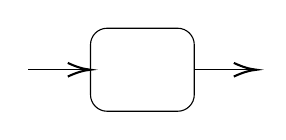
\begin{tikzpicture}[x=0.75pt,y=0.75pt,yscale=-1,xscale=1]
  %uncomment if require: \path (0,300); %set diagram left start at 0, and has height of 300

  %Rounded Rect [id:dp0789068585463999] 
  \draw   (50,28) .. controls (50,23.58) and (53.58,20) .. (58,20) -- (92,20) .. controls (96.42,20) and
  (100,23.58) .. (100,28) -- (100,52) .. controls (100,56.42) and (96.42,60) .. (92,60) -- (58,60) .. controls
  (53.58,60) and (50,56.42) .. (50,52) -- cycle ;
  %Straight Lines [id:da09494407735701005] 
  \draw    (100,40) -- (128,40) ;
  \draw [shift={(130,40)}, rotate = 180] [color={rgb, 255:red, 0; green, 0; blue, 0 }	][line width=0.75]    (10.93,-3.29) .. controls (6.95,-1.4) and (3.31,-0.3) .. (0,0) .. controls (3.31,0.3) and (6.95,1.4)
  .. (10.93,3.29)   ;
  %Straight Lines [id:da5360369763381094] 
  \draw    (20,40) -- (48,40) ;
  \draw [shift={(50,40)}, rotate = 180] [color={rgb, 255:red, 0; green, 0; blue, 0 }	][line width=0.75]    (10.93,-3.29) .. controls (6.95,-1.4) and (3.31,-0.3) .. (0,0) .. controls (3.31,0.3) and (6.95,1.4)
  .. (10.93,3.29)   ;

  % Text Node
  \draw (76,41) node   [align=left] {\Mem};

\end{tikzpicture}
\end{document}
